% Created by tikzDevice version 0.12.6 on 2024-02-25 12:47:57
% !TEX encoding = UTF-8 Unicode
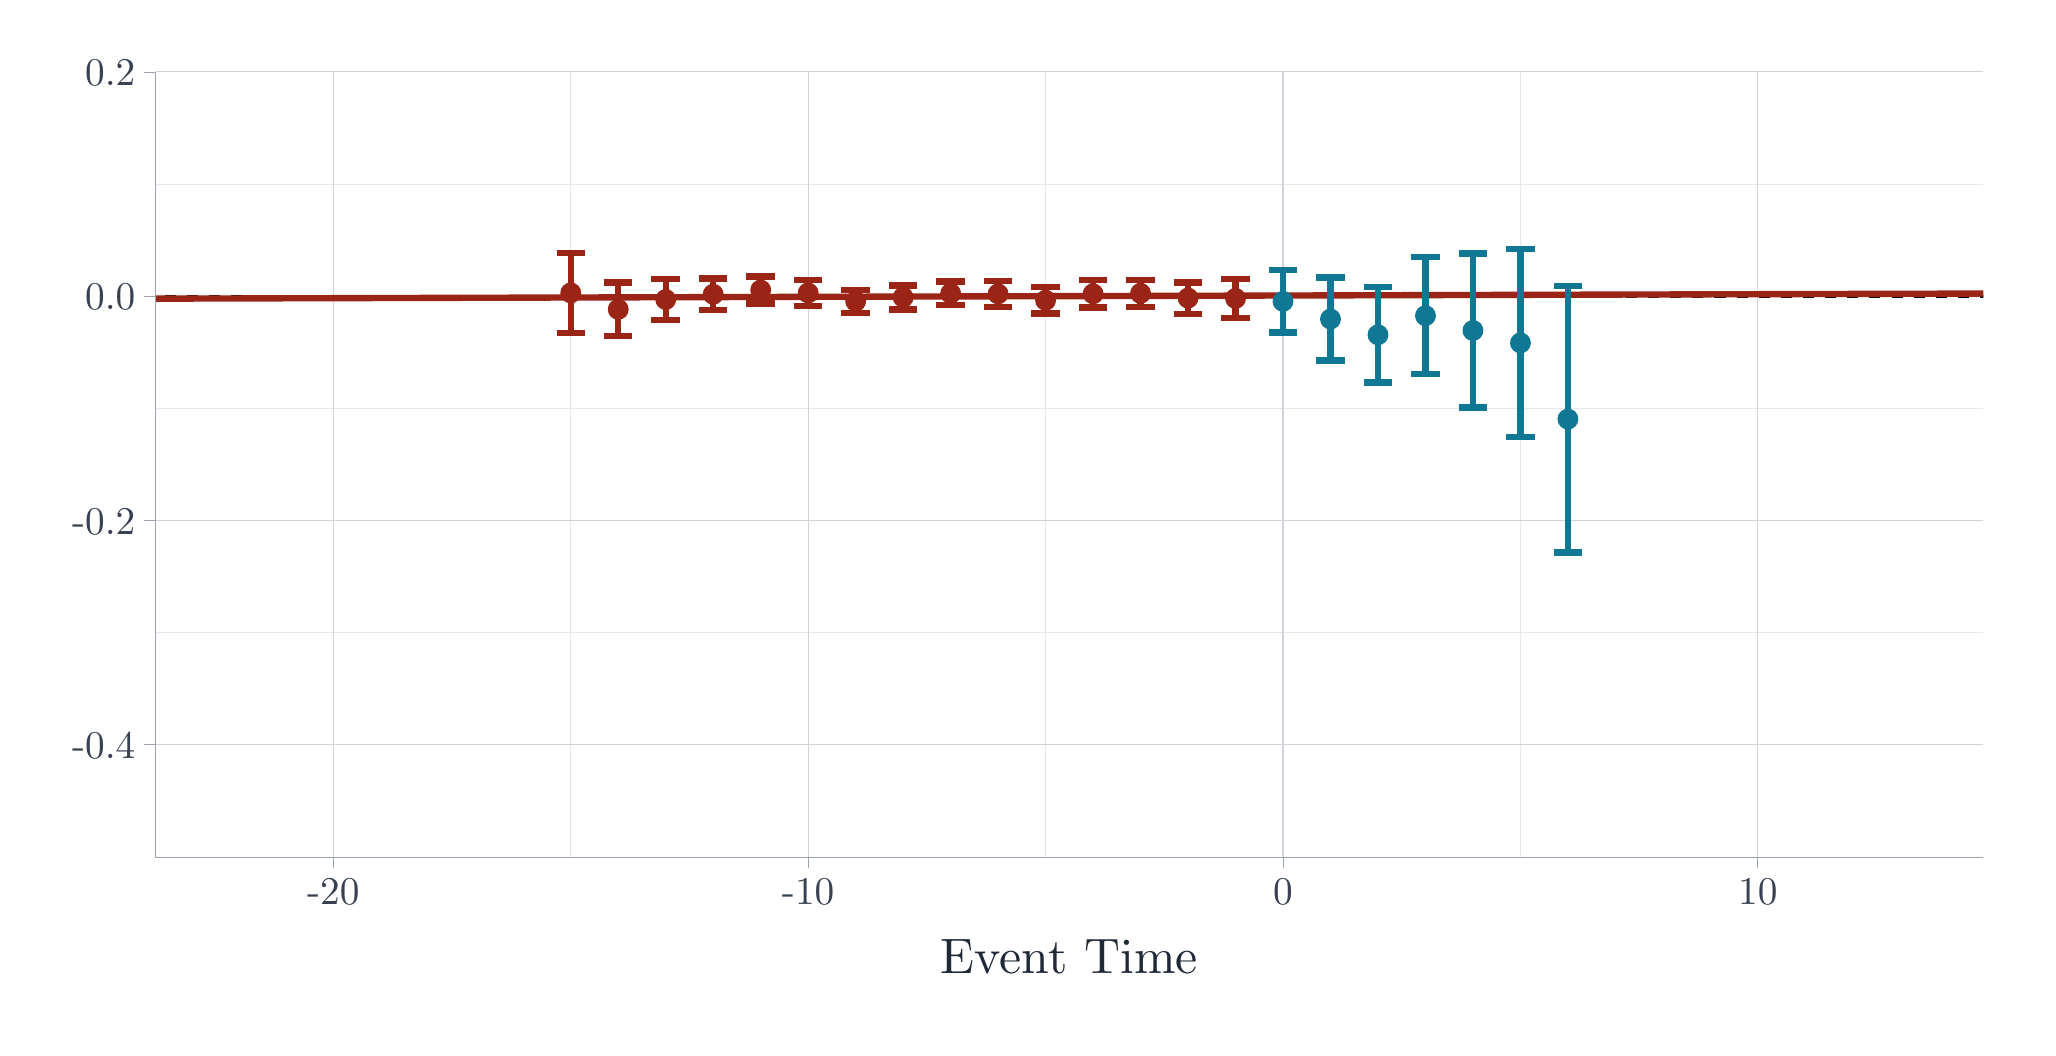
\begin{tikzpicture}[x=1pt,y=1pt]
\definecolor{fillColor}{RGB}{255,255,255}
\path[use as bounding box,fill=fillColor] (0,0) rectangle (722.70,361.35);
\begin{scope}
\path[clip] (  0.00,  0.00) rectangle (722.70,361.35);
\definecolor{drawColor}{RGB}{255,255,255}

\path[draw=drawColor,line width= 0.8pt,line join=round,line cap=round,fill=fillColor] (  0.00,  0.00) rectangle (722.70,361.35);
\end{scope}
\begin{scope}
\path[clip] ( 46.10, 61.65) rectangle (706.70,345.35);
\definecolor{drawColor}{RGB}{255,255,255}
\definecolor{fillColor}{RGB}{255,255,255}

\path[draw=drawColor,line width= 0.8pt,line join=round,line cap=round,fill=fillColor] ( 46.10, 61.65) rectangle (706.70,345.35);
\definecolor{drawColor}{RGB}{229,231,235}

\path[draw=drawColor,line width= 0.2pt,line join=round] ( 46.10,142.71) --
	(706.70,142.71);

\path[draw=drawColor,line width= 0.2pt,line join=round] ( 46.10,223.77) --
	(706.70,223.77);

\path[draw=drawColor,line width= 0.2pt,line join=round] ( 46.10,304.82) --
	(706.70,304.82);

\path[draw=drawColor,line width= 0.2pt,line join=round] (196.24, 61.65) --
	(196.24,345.35);

\path[draw=drawColor,line width= 0.2pt,line join=round] (367.82, 61.65) --
	(367.82,345.35);

\path[draw=drawColor,line width= 0.2pt,line join=round] (539.41, 61.65) --
	(539.41,345.35);
\definecolor{drawColor}{RGB}{209,213,219}

\path[draw=drawColor,line width= 0.4pt,line join=round] ( 46.10,102.18) --
	(706.70,102.18);

\path[draw=drawColor,line width= 0.4pt,line join=round] ( 46.10,183.24) --
	(706.70,183.24);

\path[draw=drawColor,line width= 0.4pt,line join=round] ( 46.10,264.29) --
	(706.70,264.29);

\path[draw=drawColor,line width= 0.4pt,line join=round] ( 46.10,345.35) --
	(706.70,345.35);

\path[draw=drawColor,line width= 0.4pt,line join=round] (110.45, 61.65) --
	(110.45,345.35);

\path[draw=drawColor,line width= 0.4pt,line join=round] (282.03, 61.65) --
	(282.03,345.35);

\path[draw=drawColor,line width= 0.4pt,line join=round] (453.61, 61.65) --
	(453.61,345.35);

\path[draw=drawColor,line width= 0.4pt,line join=round] (625.20, 61.65) --
	(625.20,345.35);
\definecolor{drawColor}{RGB}{0,0,0}

\path[draw=drawColor,line width= 0.9pt,dash pattern=on 4pt off 4pt ,line join=round] (-614.49,264.29) -- (1367.30,264.29);
\definecolor{drawColor}{RGB}{154,36,21}

\path[draw=drawColor,line width= 2.3pt,line join=round] (-614.49,261.57) -- (1367.30,267.12);
\definecolor{fillColor}{RGB}{154,36,21}

\path[draw=drawColor,line width= 0.4pt,line join=round,line cap=round,fill=fillColor] (196.24,265.50) circle (  3.57);

\path[draw=drawColor,line width= 0.4pt,line join=round,line cap=round,fill=fillColor] (213.40,259.57) circle (  3.57);

\path[draw=drawColor,line width= 0.4pt,line join=round,line cap=round,fill=fillColor] (230.56,263.12) circle (  3.57);

\path[draw=drawColor,line width= 0.4pt,line join=round,line cap=round,fill=fillColor] (247.71,265.02) circle (  3.57);

\path[draw=drawColor,line width= 0.4pt,line join=round,line cap=round,fill=fillColor] (264.87,266.54) circle (  3.57);

\path[draw=drawColor,line width= 0.4pt,line join=round,line cap=round,fill=fillColor] (282.03,265.49) circle (  3.57);

\path[draw=drawColor,line width= 0.4pt,line join=round,line cap=round,fill=fillColor] (299.19,262.49) circle (  3.57);

\path[draw=drawColor,line width= 0.4pt,line join=round,line cap=round,fill=fillColor] (316.35,263.90) circle (  3.57);

\path[draw=drawColor,line width= 0.4pt,line join=round,line cap=round,fill=fillColor] (333.51,265.32) circle (  3.57);

\path[draw=drawColor,line width= 0.4pt,line join=round,line cap=round,fill=fillColor] (350.66,265.16) circle (  3.57);

\path[draw=drawColor,line width= 0.4pt,line join=round,line cap=round,fill=fillColor] (367.82,262.84) circle (  3.57);

\path[draw=drawColor,line width= 0.4pt,line join=round,line cap=round,fill=fillColor] (384.98,265.18) circle (  3.57);

\path[draw=drawColor,line width= 0.4pt,line join=round,line cap=round,fill=fillColor] (402.14,265.35) circle (  3.57);

\path[draw=drawColor,line width= 0.4pt,line join=round,line cap=round,fill=fillColor] (419.30,263.65) circle (  3.57);

\path[draw=drawColor,line width= 0.4pt,line join=round,line cap=round,fill=fillColor] (436.46,263.51) circle (  3.57);
\definecolor{drawColor}{RGB}{16,120,149}
\definecolor{fillColor}{RGB}{16,120,149}

\path[draw=drawColor,line width= 0.4pt,line join=round,line cap=round,fill=fillColor] (453.61,262.45) circle (  3.57);

\path[draw=drawColor,line width= 0.4pt,line join=round,line cap=round,fill=fillColor] (470.77,256.06) circle (  3.57);

\path[draw=drawColor,line width= 0.4pt,line join=round,line cap=round,fill=fillColor] (487.93,250.38) circle (  3.57);

\path[draw=drawColor,line width= 0.4pt,line join=round,line cap=round,fill=fillColor] (505.09,257.28) circle (  3.57);

\path[draw=drawColor,line width= 0.4pt,line join=round,line cap=round,fill=fillColor] (522.25,251.92) circle (  3.57);

\path[draw=drawColor,line width= 0.4pt,line join=round,line cap=round,fill=fillColor] (539.41,247.43) circle (  3.57);

\path[draw=drawColor,line width= 0.4pt,line join=round,line cap=round,fill=fillColor] (556.56,219.91) circle (  3.57);
\definecolor{drawColor}{RGB}{154,36,21}

\path[draw=drawColor,line width= 2.3pt,line join=round] (191.09,279.88) --
	(201.39,279.88);

\path[draw=drawColor,line width= 2.3pt,line join=round] (196.24,279.88) --
	(196.24,251.12);

\path[draw=drawColor,line width= 2.3pt,line join=round] (191.09,251.12) --
	(201.39,251.12);

\path[draw=drawColor,line width= 2.3pt,line join=round] (208.25,269.22) --
	(218.55,269.22);

\path[draw=drawColor,line width= 2.3pt,line join=round] (213.40,269.22) --
	(213.40,249.92);

\path[draw=drawColor,line width= 2.3pt,line join=round] (208.25,249.92) --
	(218.55,249.92);

\path[draw=drawColor,line width= 2.3pt,line join=round] (225.41,270.60) --
	(235.70,270.60);

\path[draw=drawColor,line width= 2.3pt,line join=round] (230.56,270.60) --
	(230.56,255.64);

\path[draw=drawColor,line width= 2.3pt,line join=round] (225.41,255.64) --
	(235.70,255.64);

\path[draw=drawColor,line width= 2.3pt,line join=round] (242.57,270.76) --
	(252.86,270.76);

\path[draw=drawColor,line width= 2.3pt,line join=round] (247.71,270.76) --
	(247.71,259.27);

\path[draw=drawColor,line width= 2.3pt,line join=round] (242.57,259.27) --
	(252.86,259.27);

\path[draw=drawColor,line width= 2.3pt,line join=round] (259.73,271.43) --
	(270.02,271.43);

\path[draw=drawColor,line width= 2.3pt,line join=round] (264.87,271.43) --
	(264.87,261.64);

\path[draw=drawColor,line width= 2.3pt,line join=round] (259.73,261.64) --
	(270.02,261.64);

\path[draw=drawColor,line width= 2.3pt,line join=round] (276.88,270.19) --
	(287.18,270.19);

\path[draw=drawColor,line width= 2.3pt,line join=round] (282.03,270.19) --
	(282.03,260.80);

\path[draw=drawColor,line width= 2.3pt,line join=round] (276.88,260.80) --
	(287.18,260.80);

\path[draw=drawColor,line width= 2.3pt,line join=round] (294.04,266.65) --
	(304.34,266.65);

\path[draw=drawColor,line width= 2.3pt,line join=round] (299.19,266.65) --
	(299.19,258.33);

\path[draw=drawColor,line width= 2.3pt,line join=round] (294.04,258.33) --
	(304.34,258.33);

\path[draw=drawColor,line width= 2.3pt,line join=round] (311.20,268.24) --
	(321.50,268.24);

\path[draw=drawColor,line width= 2.3pt,line join=round] (316.35,268.24) --
	(316.35,259.57);

\path[draw=drawColor,line width= 2.3pt,line join=round] (311.20,259.57) --
	(321.50,259.57);

\path[draw=drawColor,line width= 2.3pt,line join=round] (328.36,269.56) --
	(338.65,269.56);

\path[draw=drawColor,line width= 2.3pt,line join=round] (333.51,269.56) --
	(333.51,261.09);

\path[draw=drawColor,line width= 2.3pt,line join=round] (328.36,261.09) --
	(338.65,261.09);

\path[draw=drawColor,line width= 2.3pt,line join=round] (345.52,269.83) --
	(355.81,269.83);

\path[draw=drawColor,line width= 2.3pt,line join=round] (350.66,269.83) --
	(350.66,260.48);

\path[draw=drawColor,line width= 2.3pt,line join=round] (345.52,260.48) --
	(355.81,260.48);

\path[draw=drawColor,line width= 2.3pt,line join=round] (362.68,267.63) --
	(372.97,267.63);

\path[draw=drawColor,line width= 2.3pt,line join=round] (367.82,267.63) --
	(367.82,258.06);

\path[draw=drawColor,line width= 2.3pt,line join=round] (362.68,258.06) --
	(372.97,258.06);

\path[draw=drawColor,line width= 2.3pt,line join=round] (379.83,270.07) --
	(390.13,270.07);

\path[draw=drawColor,line width= 2.3pt,line join=round] (384.98,270.07) --
	(384.98,260.28);

\path[draw=drawColor,line width= 2.3pt,line join=round] (379.83,260.28) --
	(390.13,260.28);

\path[draw=drawColor,line width= 2.3pt,line join=round] (396.99,270.19) --
	(407.29,270.19);

\path[draw=drawColor,line width= 2.3pt,line join=round] (402.14,270.19) --
	(402.14,260.51);

\path[draw=drawColor,line width= 2.3pt,line join=round] (396.99,260.51) --
	(407.29,260.51);

\path[draw=drawColor,line width= 2.3pt,line join=round] (414.15,269.33) --
	(424.45,269.33);

\path[draw=drawColor,line width= 2.3pt,line join=round] (419.30,269.33) --
	(419.30,257.98);

\path[draw=drawColor,line width= 2.3pt,line join=round] (414.15,257.98) --
	(424.45,257.98);

\path[draw=drawColor,line width= 2.3pt,line join=round] (431.31,270.61) --
	(441.60,270.61);

\path[draw=drawColor,line width= 2.3pt,line join=round] (436.46,270.61) --
	(436.46,256.41);

\path[draw=drawColor,line width= 2.3pt,line join=round] (431.31,256.41) --
	(441.60,256.41);
\definecolor{drawColor}{RGB}{16,120,149}

\path[draw=drawColor,line width= 2.3pt,line join=round] (448.47,273.75) --
	(458.76,273.75);

\path[draw=drawColor,line width= 2.3pt,line join=round] (453.61,273.75) --
	(453.61,251.15);

\path[draw=drawColor,line width= 2.3pt,line join=round] (448.47,251.15) --
	(458.76,251.15);

\path[draw=drawColor,line width= 2.3pt,line join=round] (465.63,271.06) --
	(475.92,271.06);

\path[draw=drawColor,line width= 2.3pt,line join=round] (470.77,271.06) --
	(470.77,241.06);

\path[draw=drawColor,line width= 2.3pt,line join=round] (465.63,241.06) --
	(475.92,241.06);

\path[draw=drawColor,line width= 2.3pt,line join=round] (482.78,267.65) --
	(493.08,267.65);

\path[draw=drawColor,line width= 2.3pt,line join=round] (487.93,267.65) --
	(487.93,233.10);

\path[draw=drawColor,line width= 2.3pt,line join=round] (482.78,233.10) --
	(493.08,233.10);

\path[draw=drawColor,line width= 2.3pt,line join=round] (499.94,278.40) --
	(510.24,278.40);

\path[draw=drawColor,line width= 2.3pt,line join=round] (505.09,278.40) --
	(505.09,236.16);

\path[draw=drawColor,line width= 2.3pt,line join=round] (499.94,236.16) --
	(510.24,236.16);

\path[draw=drawColor,line width= 2.3pt,line join=round] (517.10,279.73) --
	(527.40,279.73);

\path[draw=drawColor,line width= 2.3pt,line join=round] (522.25,279.73) --
	(522.25,224.11);

\path[draw=drawColor,line width= 2.3pt,line join=round] (517.10,224.11) --
	(527.40,224.11);

\path[draw=drawColor,line width= 2.3pt,line join=round] (534.26,281.42) --
	(544.55,281.42);

\path[draw=drawColor,line width= 2.3pt,line join=round] (539.41,281.42) --
	(539.41,213.44);

\path[draw=drawColor,line width= 2.3pt,line join=round] (534.26,213.44) --
	(544.55,213.44);

\path[draw=drawColor,line width= 2.3pt,line join=round] (551.42,268.07) --
	(561.71,268.07);

\path[draw=drawColor,line width= 2.3pt,line join=round] (556.56,268.07) --
	(556.56,171.74);

\path[draw=drawColor,line width= 2.3pt,line join=round] (551.42,171.74) --
	(561.71,171.74);

\path[] ( 46.10, 61.65) rectangle (706.70,345.35);
\end{scope}
\begin{scope}
\path[clip] (  0.00,  0.00) rectangle (722.70,361.35);
\definecolor{drawColor}{RGB}{156,163,175}

\path[draw=drawColor,line width= 0.3pt,line join=round] ( 46.10, 61.65) --
	( 46.10,345.35);
\end{scope}
\begin{scope}
\path[clip] (  0.00,  0.00) rectangle (722.70,361.35);
\definecolor{drawColor}{RGB}{55,65,81}

\node[text=drawColor,anchor=base east,inner sep=0pt, outer sep=0pt, scale=  1.42] at ( 38.90, 97.29) {-0.4};

\node[text=drawColor,anchor=base east,inner sep=0pt, outer sep=0pt, scale=  1.42] at ( 38.90,178.34) {-0.2};

\node[text=drawColor,anchor=base east,inner sep=0pt, outer sep=0pt, scale=  1.42] at ( 38.90,259.40) {0.0};

\node[text=drawColor,anchor=base east,inner sep=0pt, outer sep=0pt, scale=  1.42] at ( 38.90,340.45) {0.2};
\end{scope}
\begin{scope}
\path[clip] (  0.00,  0.00) rectangle (722.70,361.35);
\definecolor{drawColor}{RGB}{156,163,175}

\path[draw=drawColor,line width= 0.3pt,line join=round] ( 42.10,102.18) --
	( 46.10,102.18);

\path[draw=drawColor,line width= 0.3pt,line join=round] ( 42.10,183.24) --
	( 46.10,183.24);

\path[draw=drawColor,line width= 0.3pt,line join=round] ( 42.10,264.29) --
	( 46.10,264.29);

\path[draw=drawColor,line width= 0.3pt,line join=round] ( 42.10,345.35) --
	( 46.10,345.35);
\end{scope}
\begin{scope}
\path[clip] (  0.00,  0.00) rectangle (722.70,361.35);
\definecolor{drawColor}{RGB}{156,163,175}

\path[draw=drawColor,line width= 0.3pt,line join=round] ( 46.10, 61.65) --
	(706.70, 61.65);
\end{scope}
\begin{scope}
\path[clip] (  0.00,  0.00) rectangle (722.70,361.35);
\definecolor{drawColor}{RGB}{156,163,175}

\path[draw=drawColor,line width= 0.3pt,line join=round] (110.45, 57.65) --
	(110.45, 61.65);

\path[draw=drawColor,line width= 0.3pt,line join=round] (282.03, 57.65) --
	(282.03, 61.65);

\path[draw=drawColor,line width= 0.3pt,line join=round] (453.61, 57.65) --
	(453.61, 61.65);

\path[draw=drawColor,line width= 0.3pt,line join=round] (625.20, 57.65) --
	(625.20, 61.65);
\end{scope}
\begin{scope}
\path[clip] (  0.00,  0.00) rectangle (722.70,361.35);
\definecolor{drawColor}{RGB}{55,65,81}

\node[text=drawColor,anchor=base,inner sep=0pt, outer sep=0pt, scale=  1.42] at (110.45, 44.66) {-20};

\node[text=drawColor,anchor=base,inner sep=0pt, outer sep=0pt, scale=  1.42] at (282.03, 44.66) {-10};

\node[text=drawColor,anchor=base,inner sep=0pt, outer sep=0pt, scale=  1.42] at (453.61, 44.66) {0};

\node[text=drawColor,anchor=base,inner sep=0pt, outer sep=0pt, scale=  1.42] at (625.20, 44.66) {10};
\end{scope}
\begin{scope}
\path[clip] (  0.00,  0.00) rectangle (722.70,361.35);
\definecolor{drawColor}{RGB}{31,41,55}

\node[text=drawColor,anchor=base,inner sep=0pt, outer sep=0pt, scale=  1.80] at (376.40, 19.50) {Event Time};
\end{scope}
\end{tikzpicture}
